\documentclass{article}
\usepackage{amsmath}
\usepackage{commath}
\usepackage{siunitx}
\usepackage{graphicx}
\usepackage{geometry}
\usepackage[backend = biber, style=science]{biblatex}
\usepackage{tikz}
\usetikzlibrary{calc}
\usepackage{setspace}

\graphicspath{ {./Images/} }
\addbibresource{references.bib}

\renewcommand{\rmdefault}{ptm}

 % Package file
\geometry{a4paper, total={6in, 10in}, top=15mm, bottom=15mm}


\newcommand{\drawBorder}
{
\begin{tikzpicture}
    [remember picture, overlay] \draw[line width = 1pt] ($(current page.north west) + (0.35in, -0.35in)$) rectangle ($(current page.south east) + (-0.35in, 0.35in)$);
\end{tikzpicture}
}

%\addtocontents{toc}{\protect\thispagestyle{empty}}
%\pagenumbering{gobble}


\begin{document}

    \begin{titlepage}

    \drawBorder

    \begin{center}
        
        \vspace{1cm}

        \Huge
        \textbf{Simulation of the Two Body Problem}
        
        \vspace{5cm}
        \Large
        \textbf{Project Report By}
        
        \vspace{0.4cm}
        \huge
        \textbf{Mr. Dheeraj Vittal Shenoy}

        \vspace{4cm}

        \LARGE
        \textbf{Centre for Advanced Studies in Science and Technology (CASST)}
        \vspace{1cm}

        \begin{center}
            
\includegraphics[width=0.2\textwidth]{Logo}
        \end{center}

        \Huge
        \textbf{CANARA COLLEGE}

        \LARGE
        M.G Road, Kodialbail, Mangaluru - 575003

        \vfill
        \Large
        \textbf{October 2022}

    \end{center}


\setcounter{secnumdepth}{0}

\end{titlepage}


    \drawBorder
    \tableofcontents
    \newpage

    \vfill
\vspace*{1cm}

\section{Acknowledgement}
I would like to thank \textbf{Dhanush Vittal Shenoy}, my brother, for motivating during this project work.I would also like to thank \textbf{Luke Smith}, a youtuber, for his tutorials on \LaTeX.

    \section{Abstract}





    \section{Introduction}

\paragraph
{
    Gravitational two body problem is a classical mechanics problem of predicting the motion of two massive objects (abstractly viewed as point particles) under gravity. We make use of Newton's law of gravity and numerical methods to find the solution for the orbits of these objects, and simulate their changing positions.
}

\paragraph
{
    Let $m_1$ and $m_2$ be the masses of two massive objects assumed to be point particles, separated by a distance $r$. We assume that the gravitational interaction is only with these two bodies, and there are no bodies nearby other than the two under consideration.
}

\paragraph
{
    From Newton's law of gravity, the force $F$ experienced by an object of mass $m$ due to another object of mass $M$ separated by a distance of $R$ is given by,\\\\
}
\begin{equation}
    F = \frac{G M m}{R^2}
\end{equation}

\paragraph{
    Where $G$ is the Universal gravitational constant, having the value of
    $\SI{6.674e-11}{\newton \metre^2 \per \kg ^2}$
}

\paragraph{
    In vector form, this equation will be
}

\begin{equation}
    \vec{F} = \frac{G M m}{\vec{\abs{R}}^{\, 2}} \hat{R}
\end{equation}

\paragraph{
    Where R is the radius vector from mass $M$ to mass $m$
}
\paragraph{
    Therefore, the gravitational force between masses $m_1$ and $m_2$ is
}

\begin{equation}\label{force_eqn}
\begin{split}
    F = \frac{G m_1 m_2}{r^2}\\
    \vec{F} = \frac{G m_1 m_2}{\vec{\abs{r_{12}}}^{\, 2}} \hat{r_{12}}
\end{split}
\end{equation}

\paragraph{
    where $r_{12}$ is the vector from $m_1$ to $m_2$, and $\hat{r_{12}}$ is the unit vector in it's direction.
}

\paragraph{
    Using Newton's second law of motion, $\vec F=m \vec a$, we can calculate the acceleration of a body. Let $\vec F_{12}$ be the force on mass $m_1$ by $m_2$, then the acceleration of mass $m_1$ will be,
}

\begin{equation}
\begin{split}
    \vec F_{12} &= m_{1}\vec a_1\\
    \vec a_1 &= \frac{\vec F_{12}}{m_1}\\
    \frac{dv_1}{dt} ={} &{} \vec{\dot{v_1}} = \frac{\vec F_{12}}{m_1}\\
\end{split}
\end{equation}

\begin{equation}
\begin{split}
\frac{d^2x_1}{dt} ={} &{} \vec{\ddot {x_1}} = \frac{\vec F_{12}}{m_1} \label{displacement_eqn}
\end{split}
\end{equation}

\paragraph{
    Integrating equation (\ref{displacement_eqn}) twice using suitable numerical integration method, we can determine the position $x(t)$ of mass $m_1$. Similar calculation can be done to find $x(t)$ of $m_2$.
}

\paragraph{
    We make use of algorithm 2.1 mentioned in \citetitle{orbital_mechanics_4ed} to compute the motion of two bodies in an inertial frame of reference. We use python programming language to compute and plot the results using the algorithm mentioned above.
}

\paragraph{
    The python code for the simulation makes use of Numpy, Scipy \& Matplotlib libraries. There are 2 versions of the code, one where the motion of the bodies are with respect to an inertial frame of reference, and the other where the motion is with respect to one of the body
}

\paragraph{
    Now we start simulating the two body problem for various initial conditions of position, velocity and mass.
}

    \section{Results}

\paragraph{\textit{NOTE}: For the simulation, we use 0.2 hour as the timestep value, if not mentioned}

\begin{enumerate}

    \item
        With Position $x_1 = 0\hat{i} + 0\hat{j}$, $x_2 = 1000\hat{i} + 0\hat{j}$ in \si{\km} and velocity $v_1 = 0\hat{i} + 0\hat{j}$, $v_2 = 60\hat{i} + 60\hat{j}$ in \si{\km \per \sec} and equal masses of mass $1e26$ kg

        \begin{figure}[h!]
            \centering
            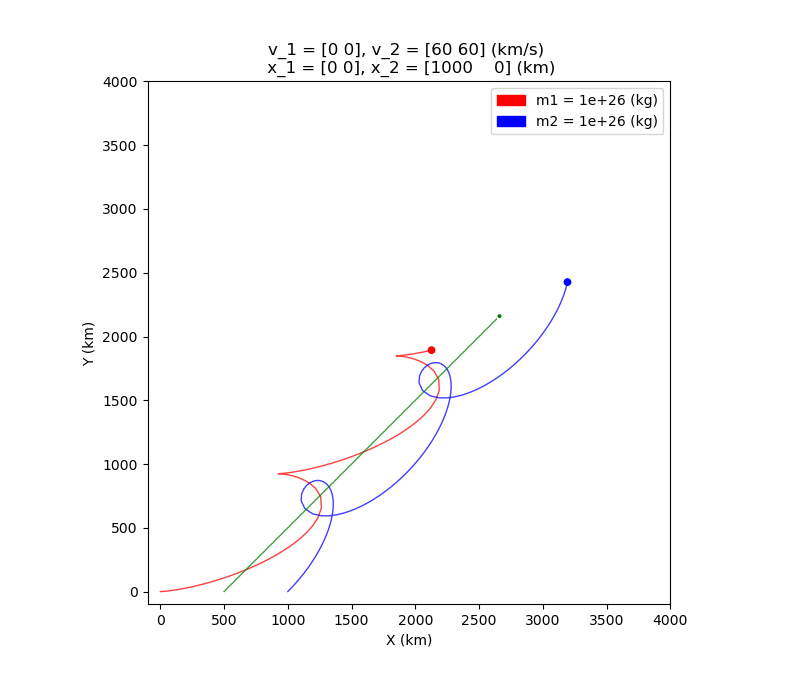
\includegraphics[width=0.8\textwidth]{fig1.png}
        \end{figure}

        This is the plot of the two body system as seen in a non-inertial frame of reference. \\The \textbf{green line} represents the center of mass of the system.

        \newpage
    \item

        With Position $x_1 = 0\hat{i} + 0\hat{j}$, $x_2 = 3000\hat{i} + 0\hat{j}$ in km and velocity $v_1 = 10\hat{i} + 20\hat{j}$, $v_2 = 0\hat{i} + 40\hat{j}$ in \si{\km \per \sec} and equal masses of mass $1e26$ kg

        \begin{figure}[h!]
            \centering
            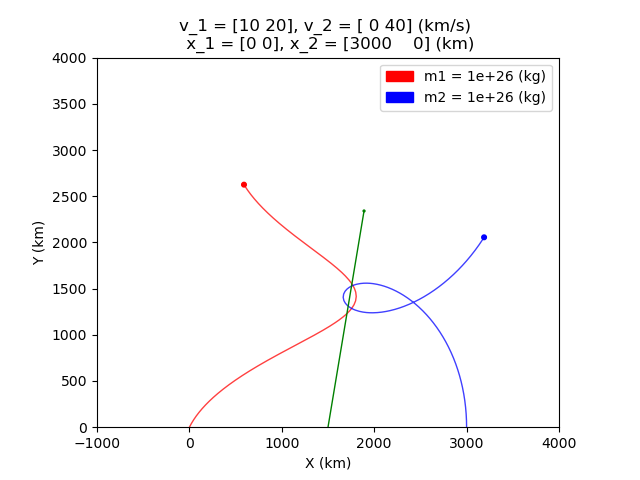
\includegraphics[width=0.8\textwidth]{fig5.png}
        \end{figure}

        Using the \textbf{Algorithm 2.2} mentioned in \textcite{orbital_mechanics_4ed} we can plot the motion of the body relative to another. The below plot shows the relative motion of $m_1$ with respect to $m_2$ using the same initial condition.

        \begin{figure}[h!]
            \centering
            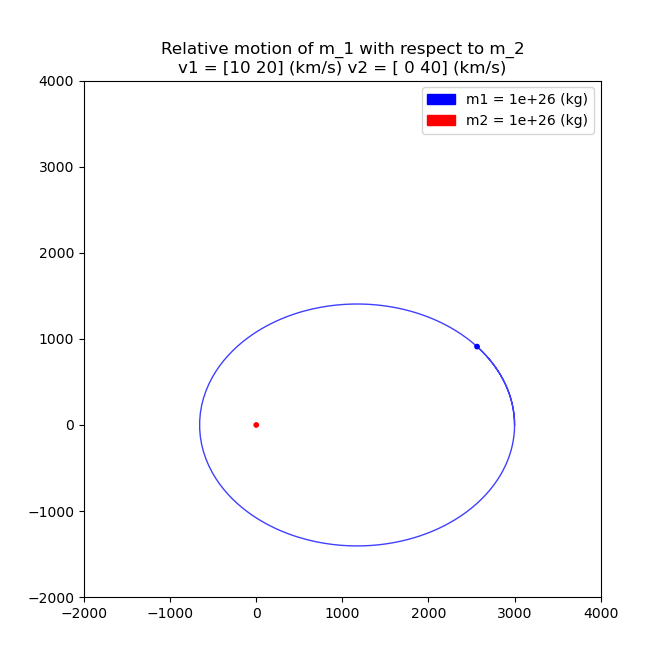
\includegraphics[width=0.7\textwidth]{fig6.png}
        \end{figure}

        \newpage
    \item
        With Position $x_1 = 500\hat{i} + 100\hat{j}$, $x_2 = 100\hat{i} + 1000\hat{j}$ in km and velocity $v_1 = 10\hat{i} + 10\hat{j}$, $v_2 = -70\hat{i} + 10\hat{j}$ in \si{\km \per \sec} and equal masses of mass $1e26$ kg

        \begin{figure}[h!]
            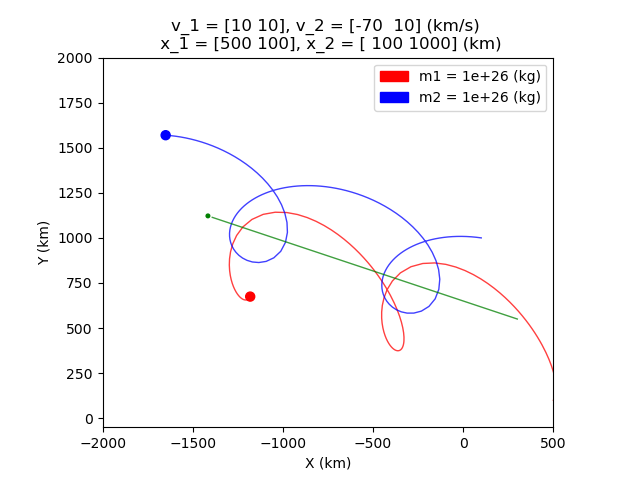
\includegraphics[width=0.8\textwidth]{fig2.png}
            \centering
        \end{figure}

        And motion of $m_1$ relative to $m_2$,

        \begin{figure}[h!]
            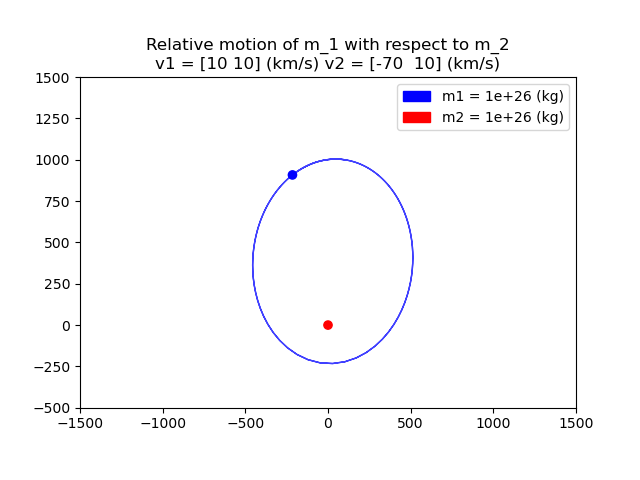
\includegraphics[width=0.8\textwidth]{fig7.png}
            \centering
        \end{figure}


        \newpage
    \item
        With Position $x_1 = 0\hat{i} + 0\hat{j}$, $x_2 = 1000\hat{i} + 1000\hat{j}$ in \si{\km} and velocity $v_1 = 0\hat{i} + 0\hat{j}$, $v_2 = -30\hat{i} + 10\hat{j}$ \si{\km \per \sec} and masses $m_1 = 1e26$ kg and $m_2 = 1e23$ kg

        \begin{figure}[h!]
            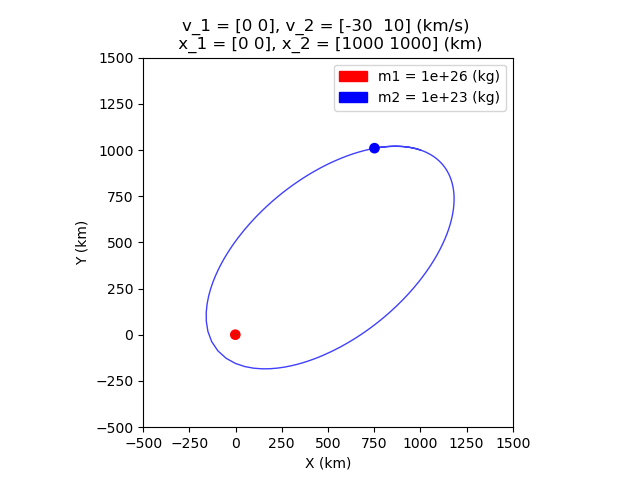
\includegraphics[width=0.8\textwidth]{fig3.png}
            \centering
        \end{figure}

        These conditions allow for a stable orbit of mass $m_2$ around $m_1$ shown in the above plot.

\end{enumerate}

    \newpage
\section{References}

\nocite{wiki_twoBodyProblem}
\nocite{modelling_n_body}
\nocite{orbital_mechanics}
\nocite{python_manual}
\nocite{matplotlib_cite}
\nocite{numpy_cite}
\nocite{scipy_cite}

\printbibliography[heading=subbibintoc, title = {Books}, type = {book}]
\printbibliography[heading=subbibintoc, title = {Articles}, type = {online}]
\printbibliography[heading=subbibintoc, title = {Libraries}, keyword = {lib}]



\end{document}
